\chapter{Mesquite Wrapper Descriptions}
\label{sec:wrappers}

Applications which desire to access Mesquite capabilities without delving 
into the low-level API can invoke wrappers to perform basic mesh quality 
improvement tasks that, except for a few user-defined inputs, are fully 
automatic. The wrappers target classic mesh optimization problems that occur 
repeatedly across many applications. See section 3.1.3 for an example of how
to invoke a wrapper. 
This chapter provides a summary of the current Mesquite wrappers. \newline

\noindent Note that the wrappers do not, by themselves, completely define
the optimization problem.  The user still has to set the fixed/free flags,
and the values of the termination criteria.  \newline

\section{Laplace-smoothing} \label{sec:LaplaceWrapper}

\noindent {\it Name}: LaplaceWrapper \newline
\noindent {\it Purpose}: Produce a {\it smooth} mesh. \newline
\noindent {\it Notes}: This is a local patch relaxation-solver. A 'smart' 
Laplacian solver is also available in Mesquite, but it is not used in this 
wrapper.  \newline
\noindent {\it Limitations/assumptions}: No invertibility guarantee. \newline 
\noindent {\it Input Termination Criterion}: Stop after 10 global iterations. \newline \newline

\noindent Under the Cover: \newline
\noindent {\it Hardwired Parameters}: None \newline
\noindent {\it Mesh/Element Type}: Any supported type. \newline
\noindent {\it Global/Local}: Local Patch with Culling \newline

\noindent Example: \newline

\begin{verbatim}
************** QualityAssessor(free only) Summary **************

  Evaluating quality for 64 elements.
  This mesh had 64 quadrilateral elements.
  THERE ARE 28 INVERTED ELEMENTS.
  (Elements invalid at 108 of 256 sample locations.)

  28 OF 64 ENTITIES EVALUATED TO AN UNDEFINED VALUE FOR Condition Number

          metric     minimum     average         rms     maximum    std.dev.
Condition Number     2.06667      437501      661438      1e+006      496077
     Edge Length     1.62019      1.8649     1.88746     2.57391    0.290915


************** QualityAssessor(free only) Summary **************

  Evaluating quality for 64 elements.
  This mesh had 64 quadrilateral elements.
  There were no inverted elements detected.
  No entities had undefined values for any computed metric.

          metric     minimum     average         rms     maximum    std.dev.
Condition Number           1           1           1           1           0
     Edge Length    0.999994           1           1           11.94596e-006
\end{verbatim}
\begin{figure*}[htbp]
\begin{center}
    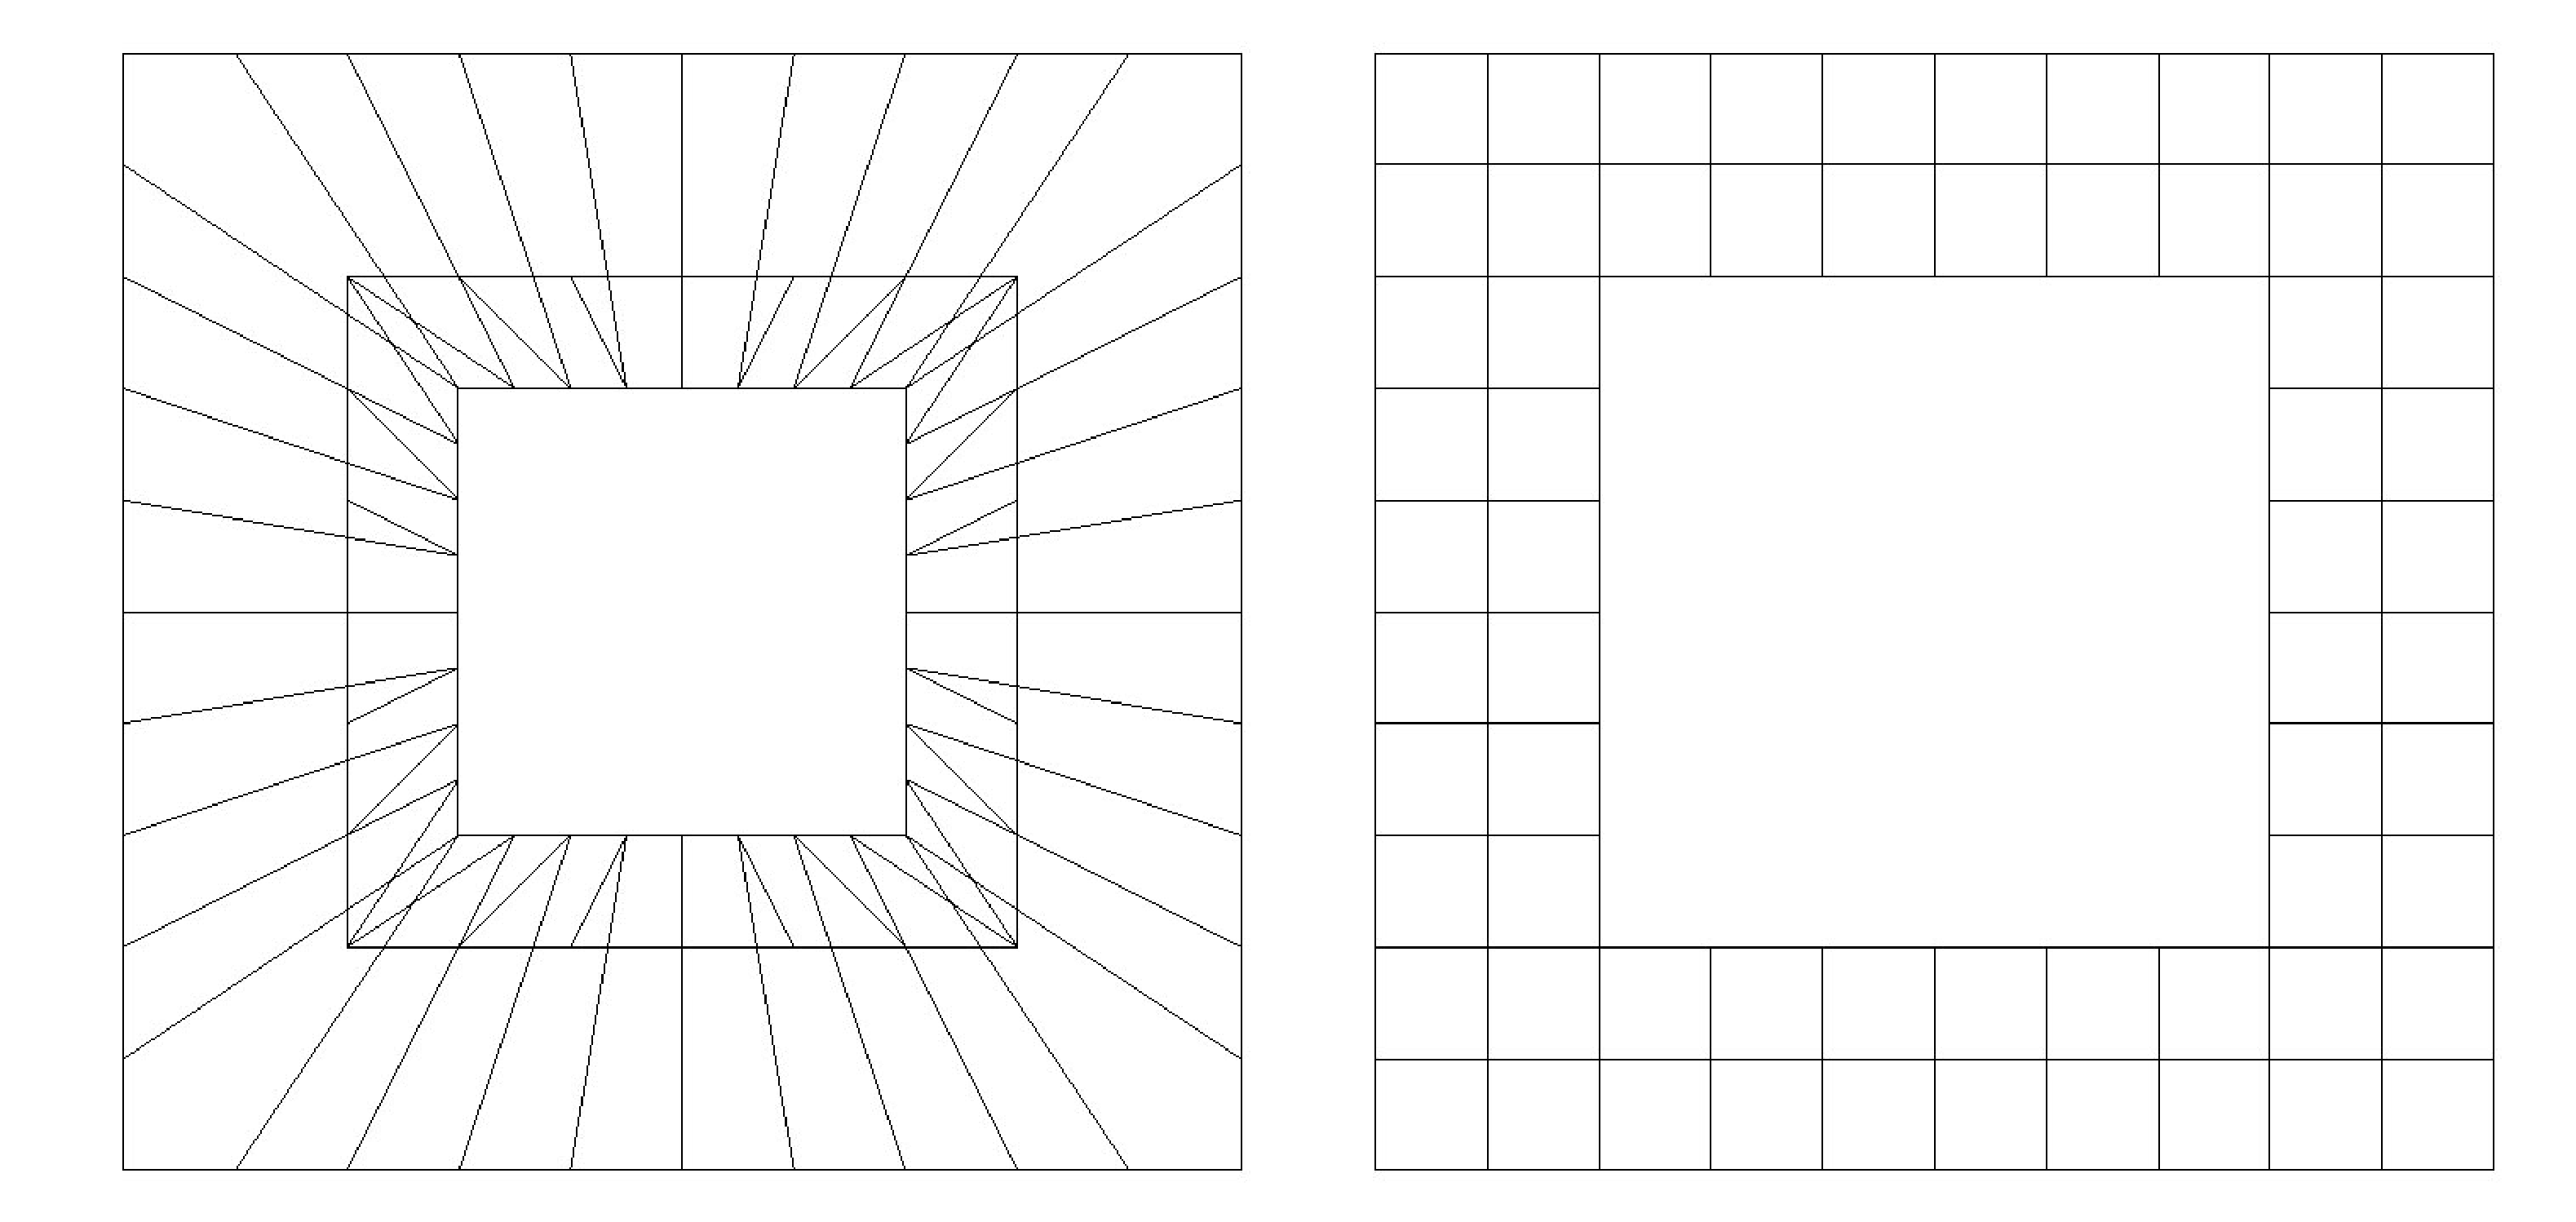
\includegraphics[height=75mm]{inverted-hole-1.eps}
    \caption{LaplaceWrapper, file: inverted-hole-1.vtk mesh. The original mesh is on the left, the mesh smoothed with the \texttt{LaplacianSmoother} is shown on the right.}
    \label{fig:inverted_hole_1}
\end{center}
\end{figure*}

\newpage

\section{Shape-Improvement} \label{sec:ShapeImprover}

\noindent {\it Name}: ShapeImprover \newline
\noindent {\it Purpose}: Make the shape of an element as close as possible to 
that of the ideal/regular element shape. For example, make triangular and 
tetrahedral elements equilateral.  The wrapper will use a non-barrier metric on meshes that contain inverted elements
and will use a barrier metric if the mesh does not contain inverted elements.  The default CPU time limit is 300 seconds.\newline 
\noindent {\it Notes}: There is no guarantee that the wrapper will be able to successfully untangle a mesh that contains inverted elements.\newline
\noindent {\it Limitations/assumptions}:  \newline 
\noindent {\it Input Termination Criterion}: CPU time limit of 300 seconds or maximum absolute vertex movement of 10 percent of the minimum edge length. \newline \newline

\noindent Under the Cover: \newline
\noindent {\it Metric}: TMPQualityMetric(Shape/ShapeBarrier) \newline
\noindent {\it Objective Function}: Algebraic mean of quality metric values \newline
\noindent {\it Mesh/Element Type}: Any supported type. \newline
\noindent {\it Solver}: Conjugate Gradient \newline
\noindent {\it Global/Local}: Global \newline

\noindent Example: \newline

\begin{verbatim}
************** QualityAssessor(free only) Summary **************

  Evaluating quality for 40 elements.
  This mesh had 40 quadrilateral elements.
  There were no inverted elements detected.
  No entities had undefined values for any computed metric.

             metric     minimum     average         rms     maximum    std.dev.
ElementPMeanP(TShapeB1)
                      0.0767863    0.232261    0.262717    0.404594    0.122781

************** QualityAssessor(free only) Summary **************

  Evaluating quality for 40 elements.
  This mesh had 40 quadrilateral elements.
  There were no inverted elements detected.
  No entities had undefined values for any computed metric.

             metric     minimum     average         rms     maximum    std.dev.
ElementPMeanP(TShapeB1)
                       0.124926    0.204118    0.207417    0.328688   0.0368497
\end{verbatim}

\begin{figure*}[htbp]
\begin{center}
    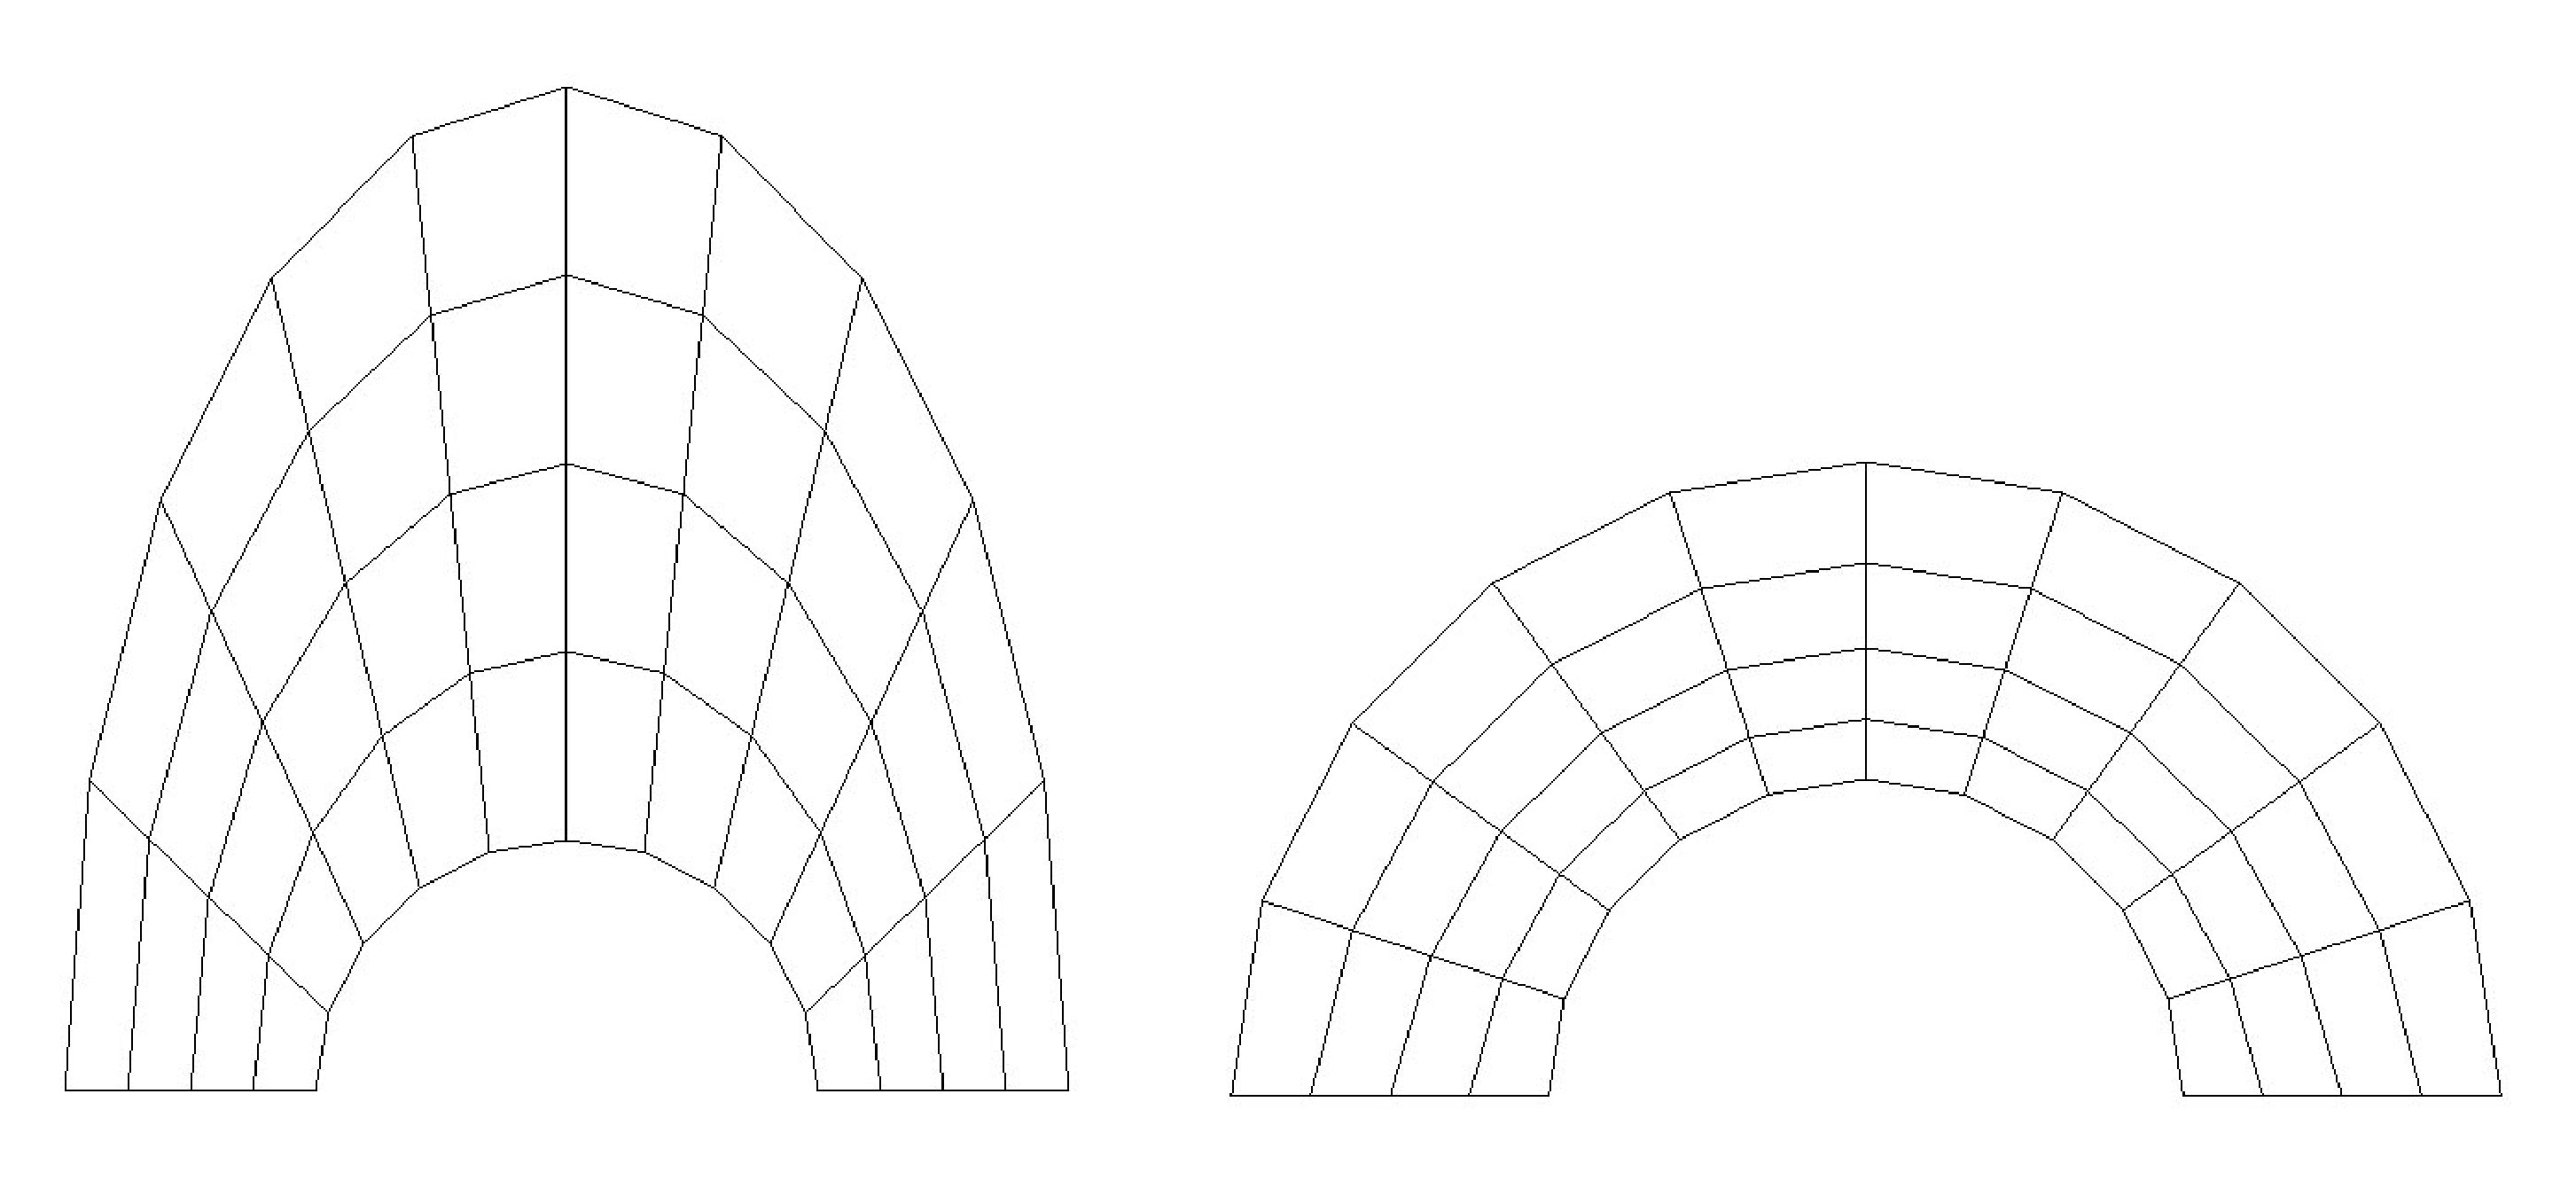
\includegraphics[height=80mm]{horseshoe-10x4.eps}
    \caption{ShapeImproverWrapper, file: tfi\_horse10x4-12.vtk mesh. The original mesh is on the left, the improved mesh is shown on the right.}
    \label{fig:inverted-hole-1}
\end{center}
\end{figure*}

\newpage

\section{Untangler} \label{sec:Untangler}

\noindent {\it Name}: UntangleWrapper \newline
\noindent {\it Purpose}: Untangle elements.  Prioritizes untangling over
element shape or other mesh quality measures.  \newline
\noindent {\it Notes}: A second optimization to improve element quality
after untangling is often necessary.  \newline
\noindent {\it Limitations/assumptions}: There is no guarantee that the optimal mesh computed using this wrapper will, in fact, be untangled.  \newline 
\noindent {\it Input Termination Criterion}: CPU time limit (not used if input 
value is non-positive) or fraction of mean edge length (default is 0.005).  It
also terminates if all elements are untangled, such that it should not modify
an input mesh with no inverted elements. \newline \newline

\noindent Under the Cover: \newline
\noindent {\it Metric}: TUntangleBeta or TUntangleMu(TSizeNB1) or TUntangleMu(TShapeSizeNB1) \newline
\noindent {\it Objective Function}: Algebraic mean of quality metric values \newline
\noindent {\it Mesh/Element Type}: Any supported type. \newline
\noindent {\it Solver}: Steepest Descent \newline
\noindent {\it Global/Local}: Local with culling, optionally Jacobi \newline

\noindent Example: \newline

\begin{verbatim}
**********************************************
Running "shest_grid32.vtk" for SHAPESIZE
**********************************************

************** QualityAssessor(free only) Summary **************

  Evaluating quality for 1024 elements.
  This mesh had 1024 quadrilateral elements.
  THERE ARE 9 INVERTED ELEMENTS.
  (Elements invalid at 9 of 4096 sample locations.)

  No entities had undefined values for any computed metric.

             metric     minimum     average         rms     maximum    std.dev.
ElementPMeanP(untangle(2D:TShapeSize2DNB1; 3D:TShapeSize3DNB1))
                              0     48.5379     210.965     2915.69     205.305

************** QualityAssessor(free only) Summary **************

  Evaluating quality for 1024 elements.
  This mesh had 1024 quadrilateral elements.
  There were no inverted elements detected.
  No entities had undefined values for any computed metric.

             metric     minimum     average         rms     maximum    std.dev.
ElementPMeanP(untangle(2D:TShapeSize2DNB1; 3D:TShapeSize3DNB1))
                              0     1.46636     23.8476     462.591     23.8025
\end{verbatim}


\begin{figure*}[htbp]
\begin{center}
    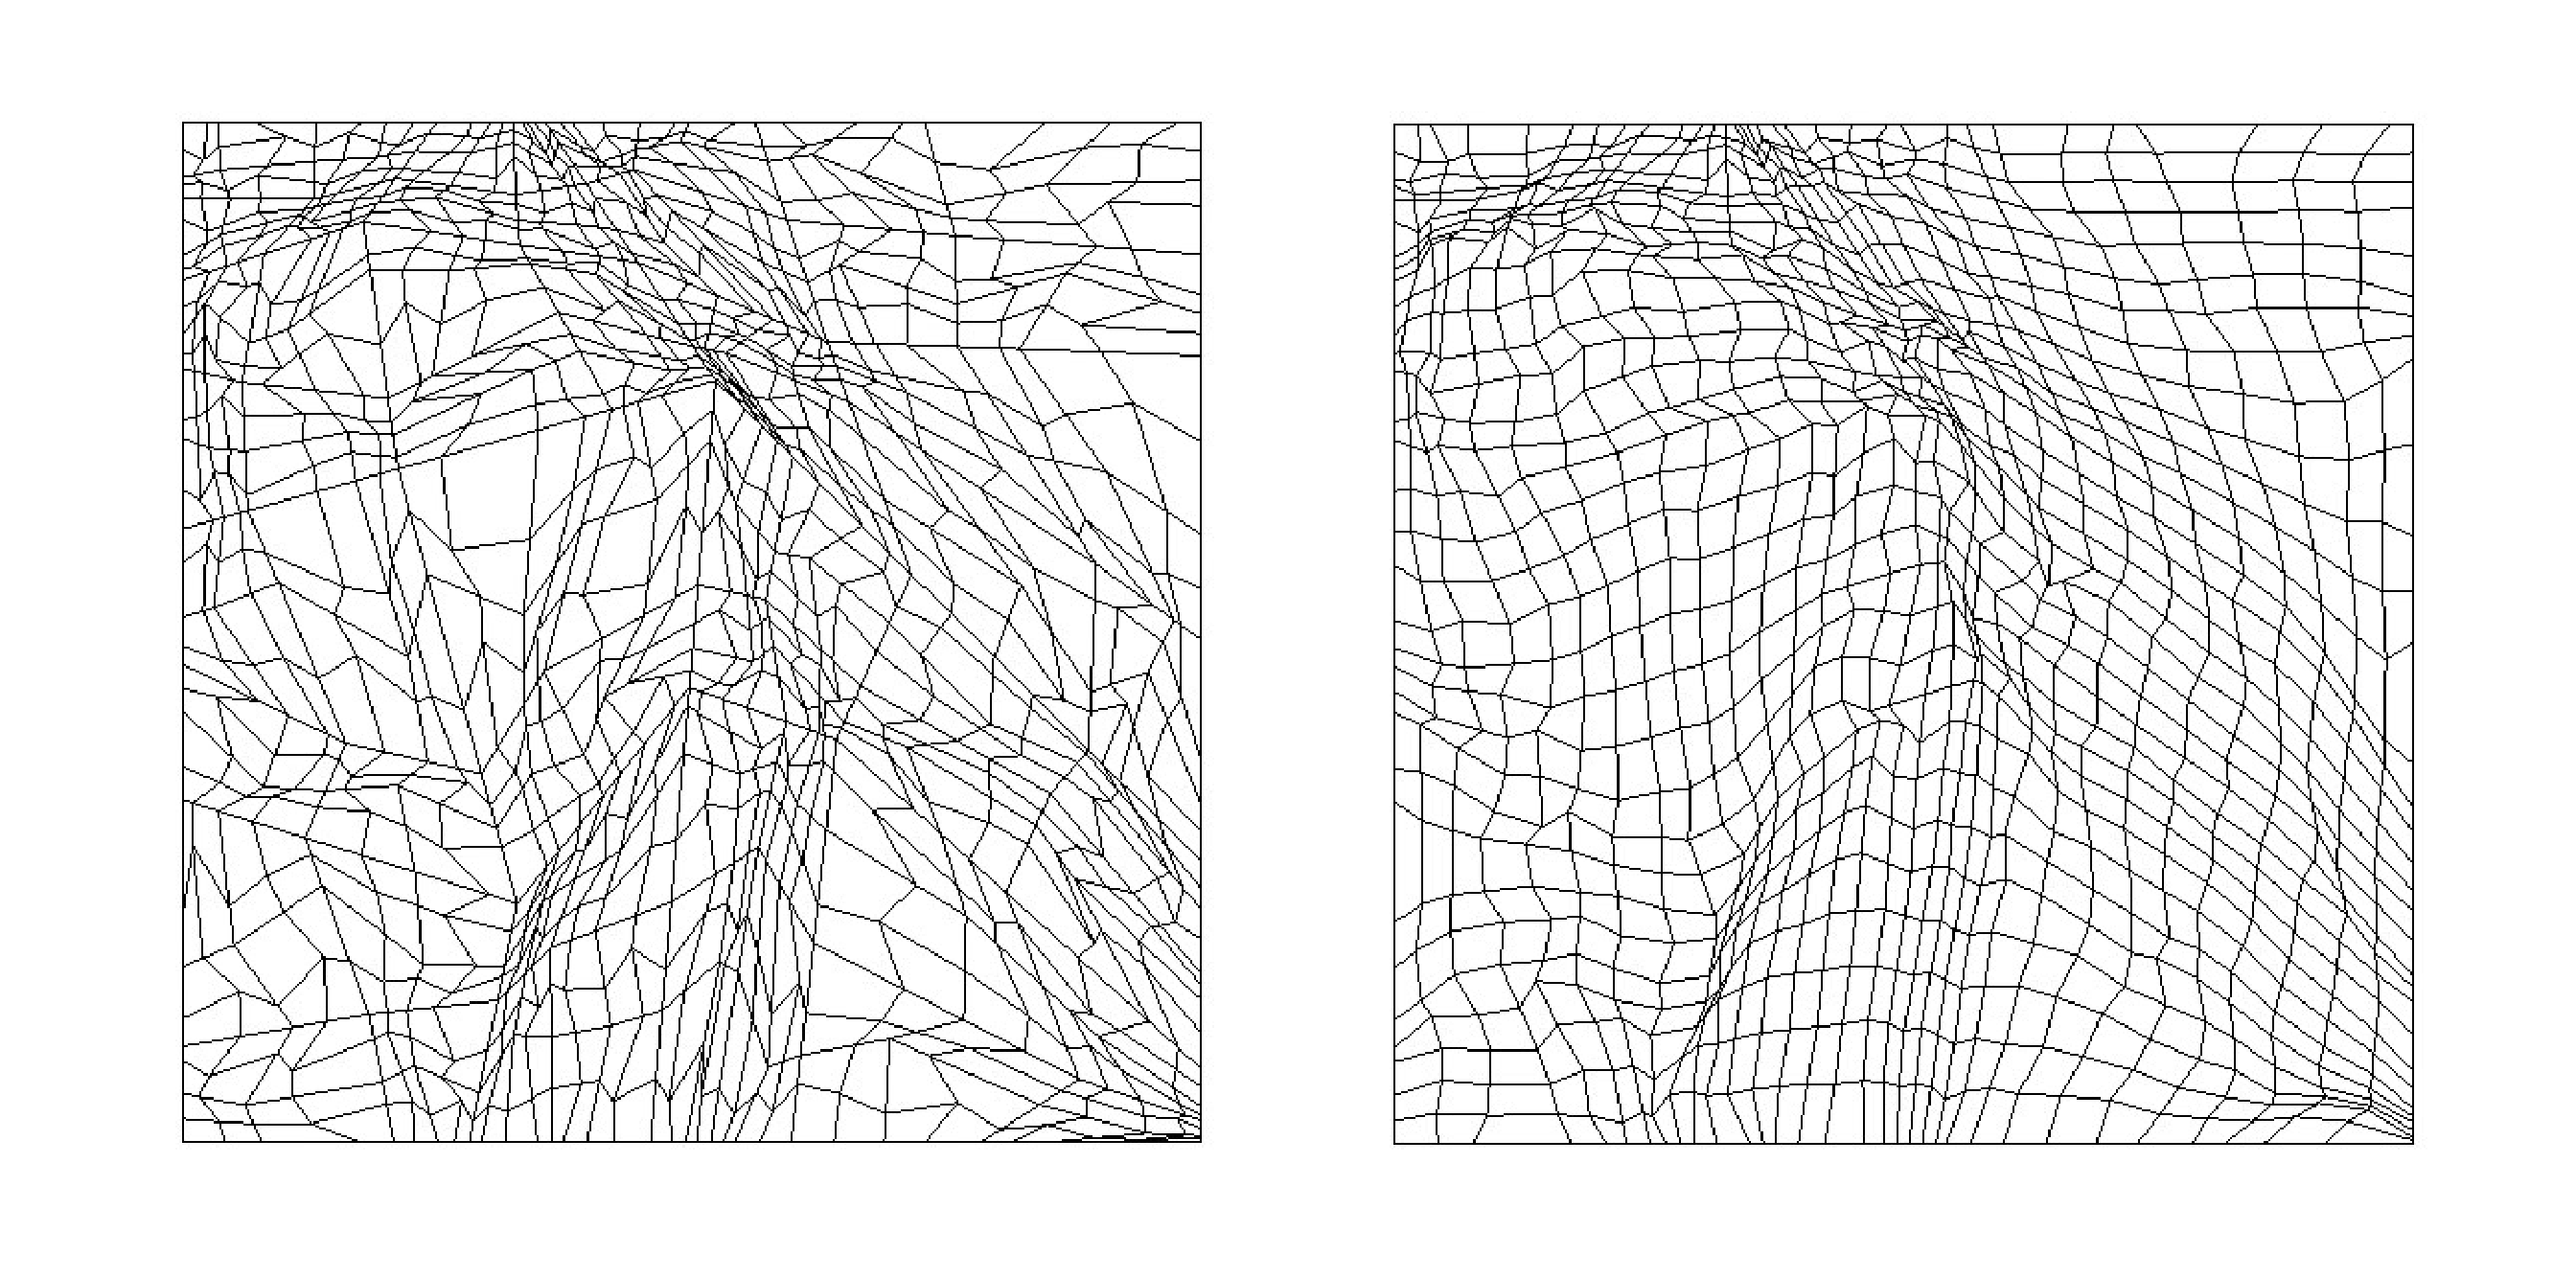
\includegraphics[height=80mm]{shest_grid32.eps}
    \caption{UntangleWrapper, TShapeSizeNB1 option, file: shest\_grid32.vtk mesh. The original mesh is on the left, the untangled mesh is shown on the right.}
    \label{fig:shest_grid32}
\end{center}
\end{figure*}

\newpage

\section{Minimum Edge-Length Improvement} \label{sec:PaverMinEdgeLengthWrapper}

\noindent {\it Name}: PaverMinEdgeLengthWrapper \newline
\noindent {\it Purpose}: Make all the edges in the mesh of equal length while 
moving toward the ideal shape. Intended for explicit PDE codes whose 
time-step limination is governed by the minimum edge-length in the mesh. \newline
\noindent {\it Notes}: Based on Target-matrix paradigm. \newline
\noindent {\it Limitations/assumptions}: Initial mesh must be non-inverted. User does not want to preserve or create anisotropic elements. \newline 
\noindent {\it Input Termination Criterion}: maximum iterations (default=50), maximum absolute vertex movement \newline \newline

\noindent Under the Cover: \newline
\noindent {\it Hardwired Parameters}: None \newline
\noindent {\it Metric}:  Target2DShapeSizeBarrier or Target3DShapeSizeBarrier \newline
\noindent {\it Tradeoff Coefficient}: 1.0 \newline
\noindent {\it Objective Function}: Linear Average over the Sample Points \newline
\noindent {\it Mesh/Element Type}: Any supported type.  \newline
\noindent {\it Solver}: Trust Region \newline
\noindent {\it Global/Local}: Global \newline

\noindent Example: \newline

\begin{verbatim}
************** QualityAssessor(free only) Summary **************

  Evaluating quality for 8 elements.
  This mesh had 8 quadrilateral elements.
  There were no inverted elements detected. 
  No entities had undefined values for any computed metric.

                     metric     minimum     average         rms     maximum    std.dev.
ElementPMeanP(TShapeSizeB1)    0.357275    0.983461     1.33806     3.27555    0.907303
                 EdgeLength    0.538516     1.11317     1.15398     1.51327    0.304184

************** QualityAssessor(free only) Summary **************

  Evaluating quality for 8 elements.
  This mesh had 8 quadrilateral elements.
  There were no inverted elements detected. 
  No entities had undefined values for any computed metric.

                     metric     minimum     average         rms     maximum    std.dev.
ElementPMeanP(TShapeSizeB1)  0.00135009   0.0017804  0.00179488  0.00221721 0.000227498
                 EdgeLength    0.994086      1.0004     1.00041     1.00293  0.00253389
\end{verbatim}


\begin{figure*}[htbp]
\begin{center}
    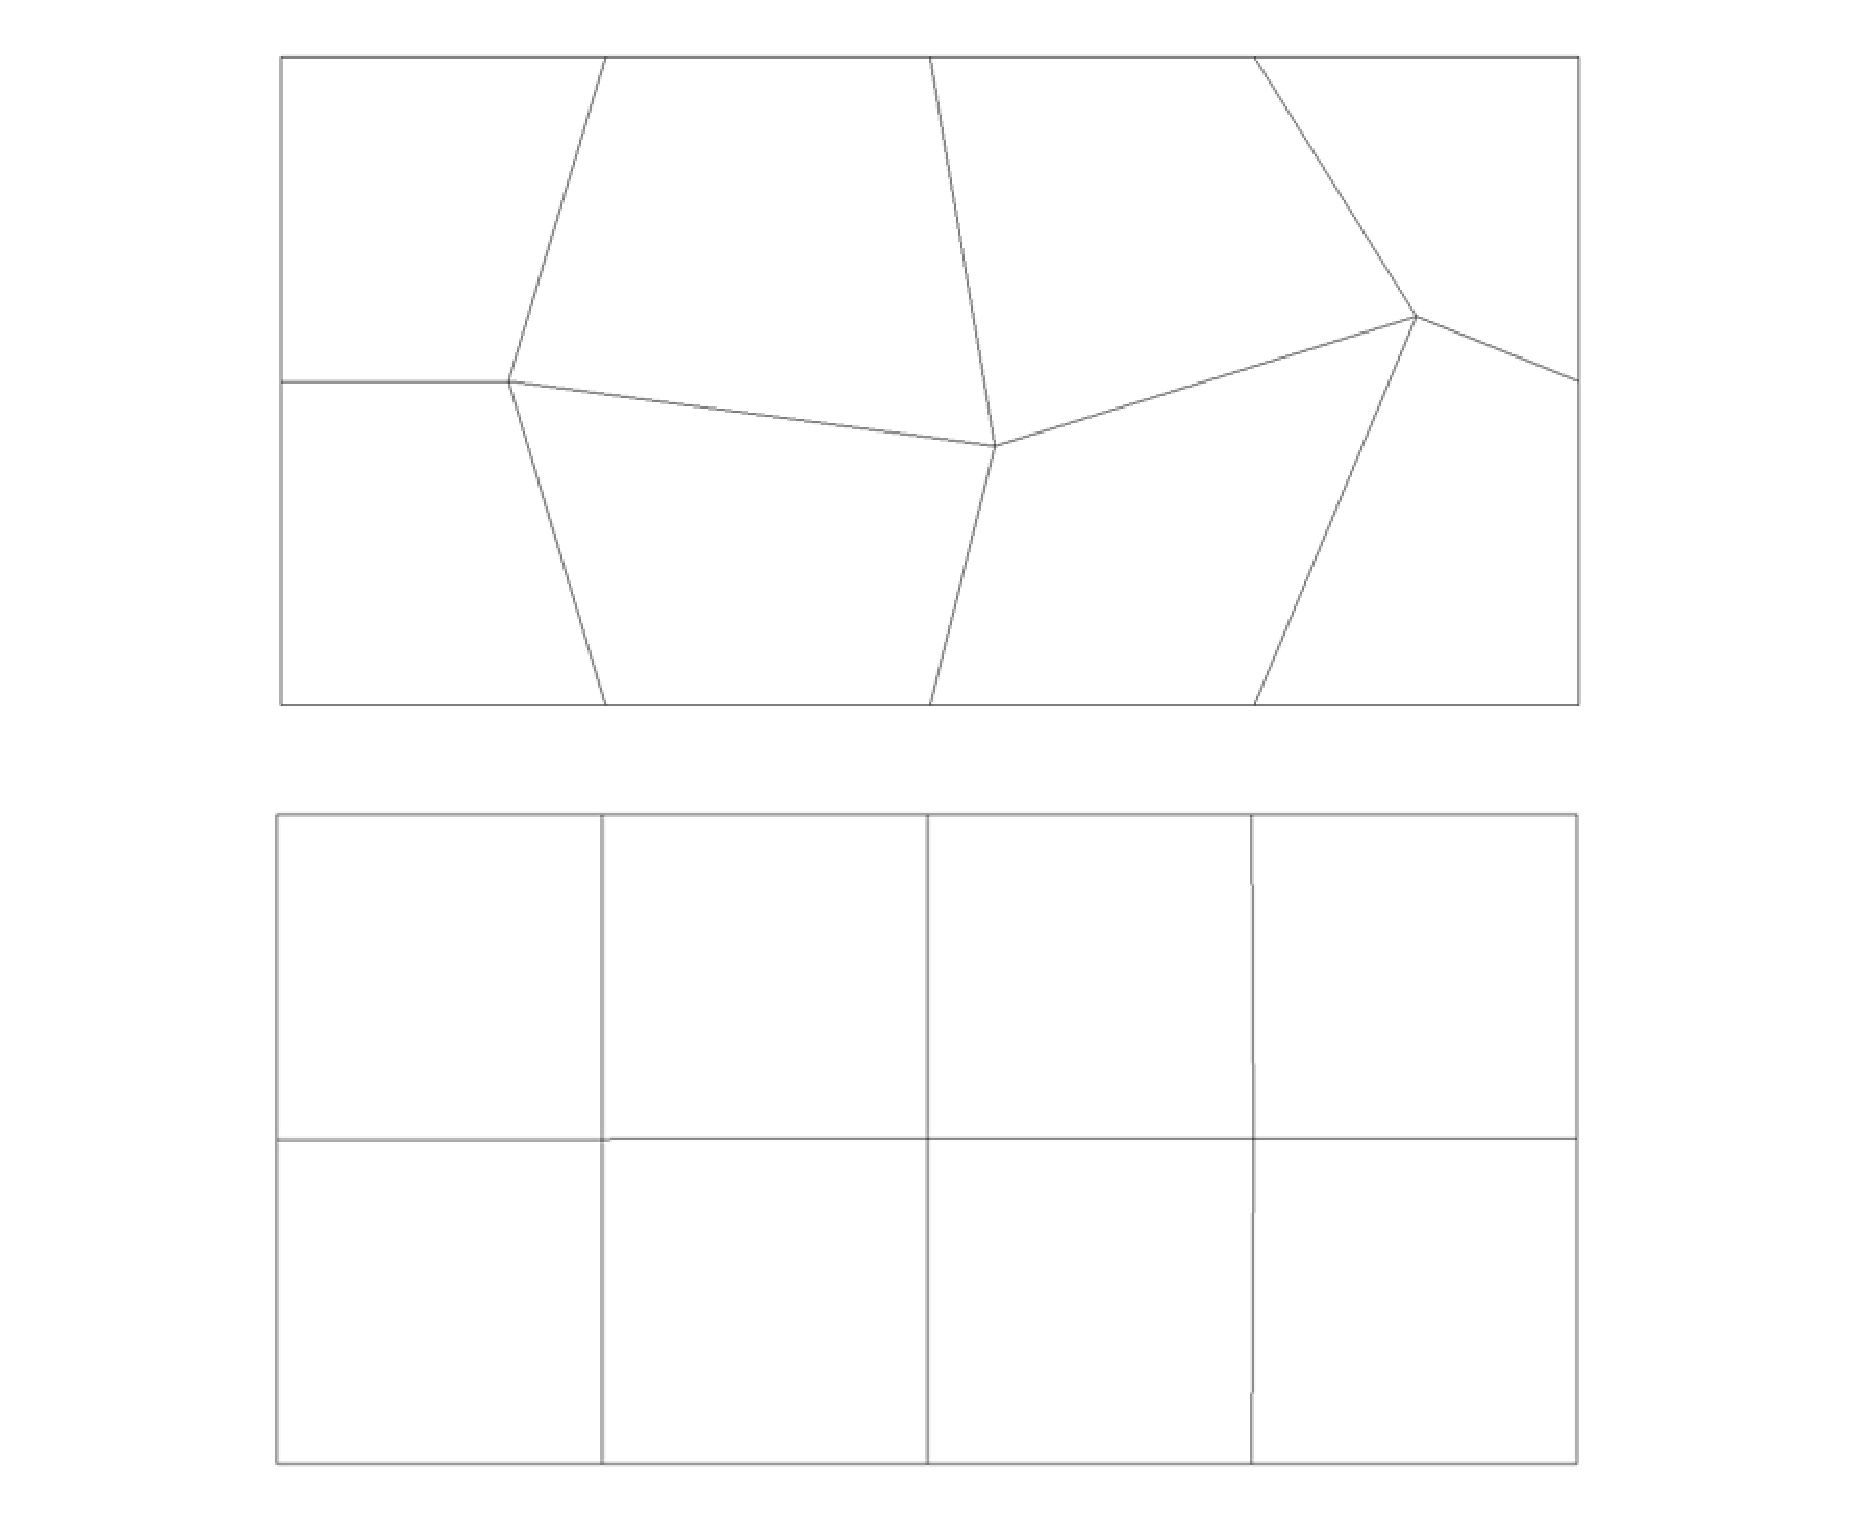
\includegraphics[height=100mm]{min-edge-length.eps}
    \caption{PaverMinEdgeLengthWrapper, file: quads\_4by2\_bad.vtk mesh. The original mesh is on the top, the improved mesh is shown on the bottom.}
    \label{fig:min_edge-length}
\end{center}
\end{figure*}
 
\newpage

\section{Improve the Shapes in a Size-adapted Mesh} \label{sec:SizeAdaptShapeWrapper}

\noindent {\it Name}: SizeAdaptShapeWrapper \newline
\noindent {\it Purpose}: Make the shape of an element as close as possible to that
of the ideal element shape, {\it while preserving, as much as possible, the size of each element in the mesh}. To be used on isotropic initial meshes that are already size-adapted. \newline
\noindent {\it Notes}: Based on Target-matrix Paradigm. \newline
\noindent {\it Limitations/assumptions}: Initial mesh must be non-inverted. 
User wants to preserve sizes of elements in initial mesh and does not want to preserve or 
create anisotropic elements.  \newline 
\noindent {\it Input Termination Criterion}: maximum iterations (default=50), maximum absolute vertex movement \newline \newline

\noindent Under the Cover: \newline
\noindent {\it Hardwired Parameters}: None \newline
\noindent {\it Metric}: Target2DShapeSizeBarrier or Target3DShapeSizeBarrier \newline
\noindent {\it Tradeoff Coefficient}: 1.0 \newline
\noindent {\it Objective Function}: Linear Average over the Sample Points \newline
\noindent {\it Mesh/Element Type}: Any supported type. \newline
\noindent {\it Solver}: Trust Region \newline
\noindent {\it Global/Local}: Global \newline

\noindent Example: \newline

\begin{verbatim}
************** QualityAssessor(free only) Summary **************

  Evaluating quality for 3456 elements.
  This mesh had 3456 quadrilateral elements.
  There were no inverted elements detectedas-sphere-quads. 
  No entities had undefined values for any computed metric.

                     metric     minimum     average         rms     maximum    std.dev.
ElementPMeanP(TShapeSizeB1)  0.00447499     0.23505    0.288066    0.710249    0.166533
                 EdgeLength    0.163072    0.574857     0.62062     1.01908      0.2339


************** QualityAssessor(free only) Summary **************

  Evaluating quality for 3456 elements.
  This mesh had 3456 quadrilateral elements.
  There were no inverted elements detected. 
  No entities had undefined values for any computed metric.

                     metric     minimum     average         rms     maximum    std.dev.
ElementPMeanP(TShapeSizeB1)  0.00558463   0.0591772   0.0767815    0.303106    0.048923
                 EdgeLength    0.161144    0.562074    0.607611     1.11686    0.230789


AREAS:      Initial     Final       Difference  Change
Polar:
  Minimum:    0.035147    0.033739    0.001407    4.003825%
  Average:    0.356401    0.355561    0.000840    0.235642%
  Maximum:    0.956929    0.896340    0.060589    6.331607%
Equatorial:
  Minimum:    0.530028    0.650497    0.120469   22.728869%
  Average:    0.718328    0.763170    0.044842    6.242616%
  Maximum:    0.957685    0.896794    0.060891    6.358101%
\end{verbatim}


\begin{figure*}[htbp]
\begin{center}
    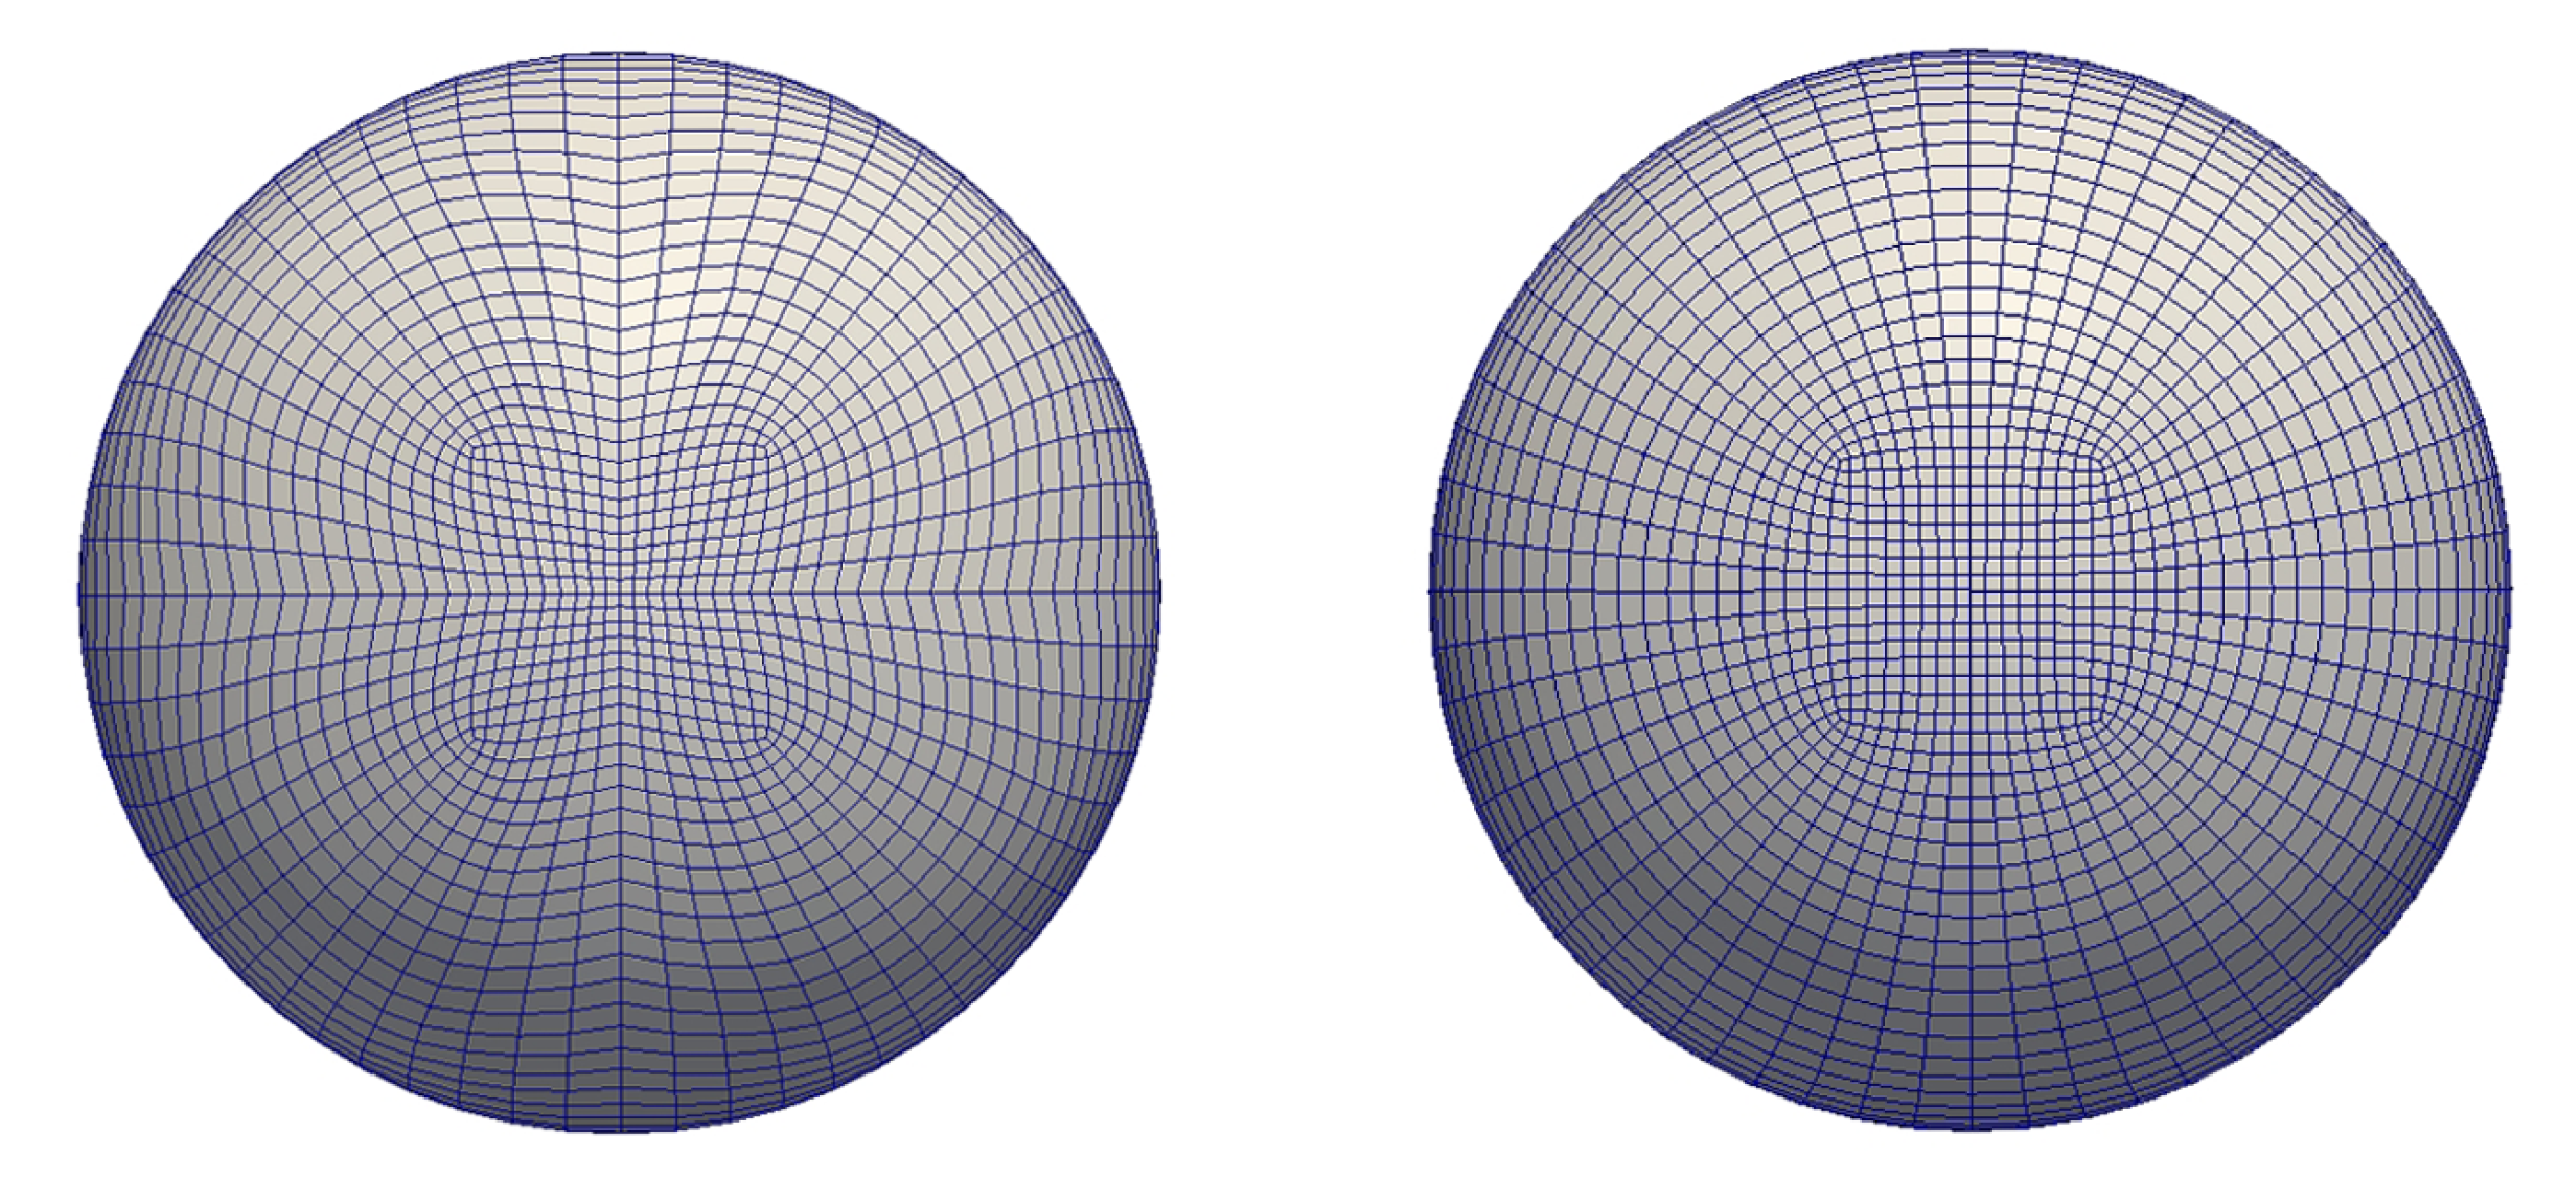
\includegraphics[height=80mm]{bias-sphere-quads.eps}
    \caption{SizeAdaptShapeWrapper, file: bias-sphere-quads.vtk mesh. The original mesh is on the left, the improved mesh is shown on the right.}
    \label{fig:shest_grid32}
\end{center}
\end{figure*}

\newpage

\section{Improve Sliver Tets in a Viscous CFD Mesh} \label{sec:ViscousCFDTetShapeWrapper}

\noindent {\it Name}: ViscousCFDTetShapeWrapper \newline
\noindent {\it Purpose}: Improve the shape of sliver elements in the far-field 
of a CFD mesh while 
preserving an existing layer of sliver elements in the boundary layer. \newline
\noindent Notes: Based on Target-matrix paradigm.  \newline
\noindent {\it Limitations/assumptions}: Tetrahedral meshes only.  \newline 
\noindent {\it Input Termination Criterion}: Iteration Count (default=50) or Maximum Absolution Vertex Movement \newline \newline
 
\noindent Under the Cover: \newline
\noindent {\it Hardwired Parameters}: In tradeoff coefficient model. \newline
\noindent {\it Metric}: Target2DShape+Target2DShapeSizeOrient (or 3D) (or Barrier) \newline
\noindent {\it Tradeoff Coefficient}: Based on element dihedral angle \newline
\noindent {\it Objective Function}: Linear average over Sample Points \newline
\noindent {\it Mesh/Element Type}: Tetrahedra \newline
\noindent {\it Solver}: Trust Region \newline
\noindent {\it Global/Local}: Global \newline


\noindent Additional Information: \newline
\noindent {\it Article}: Introducing the Target-matrix Paradigm for mesh optimization via node-movement", Engineering with Computers, Sept. 2011.\newline

\section{Deforming Domain} \label{sec:DeformingDomain}

\noindent {\it Name}: DeformingDomainWrapper \newline
\noindent {\it Purpose}:  Use initial mesh on undeformed geometric domain
to guide optimization of mesh moved to deformed geometric domain.  \newline
\noindent {\it Notes}: Uses a non-barrier metric which means that the
wrapper could potentially invert/tangle elements.  \newline
\noindent {\it Limitations/assumptions}:  Application responsible for explicit handling of mesh on geometric curves and points.  Initial mesh before moving to deformed domain must be available.\newline 
\noindent {\it Input Termination Criterion}: CPU time limit (not used if input 
value is non-positive) or fraction of mean edge length (default is 0.005). \newline \newline

\noindent Under the Cover: \newline
\noindent {\it Metric}: TMPQualityMetric(TShapeNB1 or TShapeSizeNB1 or TShapeSizeOrientNB1) \newline
\noindent {\it Objective Function}: Algebraic mean of quality metric values \newline
\noindent {\it Mesh/Element Type}: Any supported type. \newline
\noindent {\it Solver}: Steepest Descent \newline
\noindent {\it Global/Local}: Local with culling \newline

\noindent Additional Information: \newline
\noindent {\it Article}: "Updating meshes on deforming domains",  Communications in Numerical Methods in Engineering, 24:467-476, 2008..\newline

\noindent Example: \newline

\begin{verbatim}
************** QualityAssessor(free only) Summary **************

  Evaluating quality for 216 elements.
  This mesh had 216 quadrilateral elements.
  THERE ARE 56 INVERTED ELEMENTS. 
  (Elements invalid at 220 of 864 sample locations.)

  No entities had undefined values for any computed metric.

                  metric     minimum     average         rms     maximum    std.dev.
ElementPMeanP(TShapeNB1) 4.57621e-05     7.63416     20.8252     67.0217     19.3754

************** QualityAssessor(free only) Summary **************

  Evaluating quality for 216 elements.
  This mesh had 216 quadrilateral elements.
  There were no inverted elements detected. 
  No entities had undefined values for any computed metric.

                  metric     minimum     average         rms     maximum    std.dev.
ElementPMeanP(TShapeNB1) 0.000763758   0.0202682   0.0252805   0.0947676   0.0151097
\end{verbatim}


\begin{figure*}[htbp]
\begin{center}
    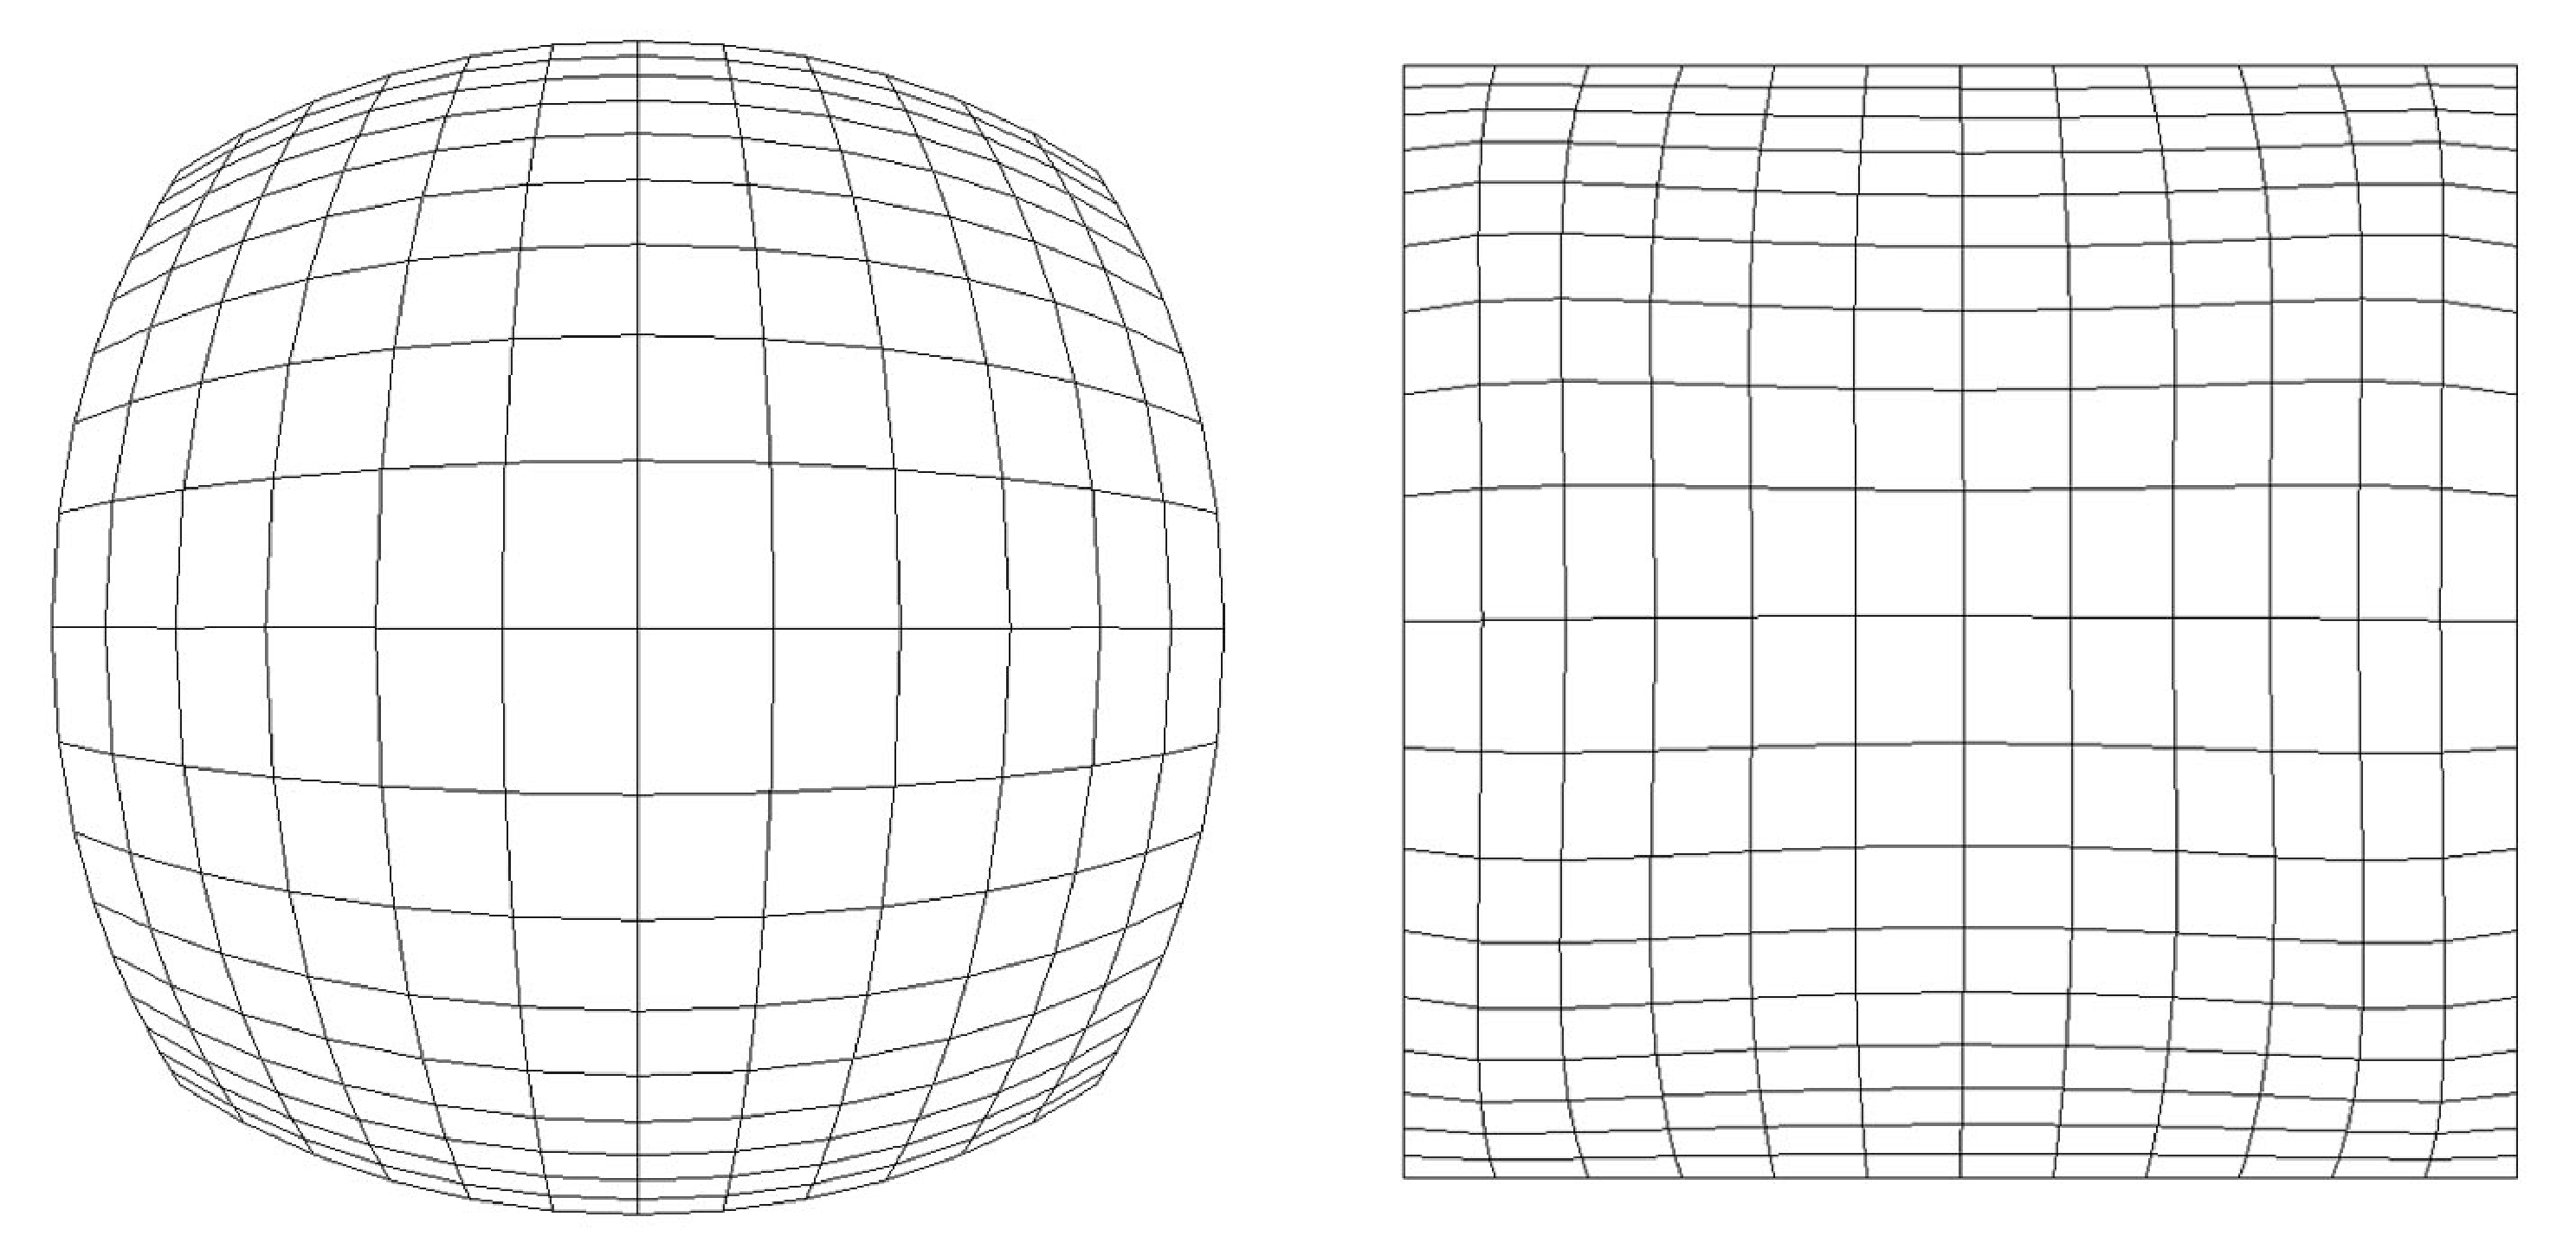
\includegraphics[height=80mm]{sph-10-zsquare.eps}
    \caption{DeformingDomainWrapper, file: sph-10-zsquare.vtk mesh. The original mesh is on the left, the improved mesh is shown on the right.}
    \label{fig:sph-10-zsquare}
\end{center}
\end{figure*}
